\documentclass[11pt,a4paper]{article}
\usepackage[utf8]{inputenc}
\usepackage[T1]{fontenc}
\usepackage{geometry}
\usepackage{graphicx}
\usepackage{booktabs}
\usepackage{multirow}
\usepackage{array}
\usepackage{xcolor}
\usepackage{amsmath}
\usepackage{hyperref}
\usepackage{fancyhdr}
\usepackage{titlesec}
\usepackage{float}
\usepackage{caption}
\usepackage{subcaption}
\usepackage{enumitem}
\usepackage{url}

% Page setup
\geometry{margin=0.8in}
\pagestyle{fancy}
\fancyhf{}
\fancyhead[L]{\leftmark}
\fancyhead[R]{VIF-Eval Benchmark Report}
\fancyfoot[C]{\thepage}

% Title formatting
\titleformat{\section}{\Large\bfseries\color{blue!70!black}}{\thesection}{1em}{}
\titleformat{\subsection}{\large\bfseries\color{blue!50!black}}{\thesubsection}{1em}{}
\titleformat{\subsubsection}{\normalsize\bfseries}{\thesubsubsection}{1em}{}

% Colors
\definecolor{primaryblue}{RGB}{0,102,204}
\definecolor{secondaryblue}{RGB}{51,153,255}
\definecolor{accentorange}{RGB}{255,153,0}

% Hyperref setup
\hypersetup{
    colorlinks=true,
    linkcolor=primaryblue,
    urlcolor=primaryblue,
    citecolor=primaryblue
}

\title{\Huge\textbf{The Visual Instruction Following Evaluation Benchmark (VIF-Eval)}\\
\Large A Comprehensive Framework for Evaluating Compositional and Editorial Image Generation\\
\vspace{0.5cm}
\large Complete Assessment Report}
\author{Evaluation Team}
\date{November 2025}

\begin{document}

\maketitle
\thispagestyle{empty}

\newpage
\tableofcontents
\newpage
\listoffigures
\newpage
\listoftables
\newpage

\section{Executive Summary}

This comprehensive report presents the complete evaluation results of the Visual Instruction Following Evaluation Benchmark (VIF-Eval), a novel framework for assessing generative visual models across multiple dimensions of real-world performance. We evaluated three state-of-the-art models—GPT Image 1, DALL-E 3, and Gemini 2.5 Flash Image (Nano Banana)—across 47 diverse prompts with 167+ constraints.

\textbf{Key Findings:}
\begin{itemize}
    \item GPT Image 1 achieves the highest overall pass rate (58.1\%)
    \item Nano Banana performs comparably (54.7\%) with significantly lower cost
    \item Models excel at spatial relationships (100\% pass rate) and CSP constraints (95-100\%)
    \item Critical weakness in text rendering (12-13\% pass rate across all models)
    \item Cost-performance analysis reveals Nano Banana as most cost-effective
\end{itemize}

\section{Introduction}

\subsection{Background}

Generative visual models have achieved remarkable progress in recent years, enabling high-quality image synthesis from text prompts. Models like DALL-E 3, Midjourney, Stable Diffusion, and GPT Image 1 have demonstrated impressive capabilities in creating photorealistic and artistic images. However, as these models are increasingly deployed in real-world applications—including e-commerce, advertising, design, and creative industries—there is a growing need to evaluate their performance beyond simple aesthetic quality.

\subsection{Motivation and Industry Relevance}

Real-world visual generation tasks often require:
\begin{enumerate}
    \item \textbf{Complex Compositional Reasoning}: Correctly placing multiple objects with specific attributes and spatial relationships
    \item \textbf{Accurate Text Rendering}: Generating legible text within images for posters, labels, and advertisements
    \item \textbf{Constraint Satisfaction}: Following mathematical and logical constraints (e.g., nutrition labels, data tables)
    \item \textbf{Consistency}: Maintaining character appearance and style across multiple scenes
    \item \textbf{Precision Editing}: Modifying specific image regions while preserving context
\end{enumerate}

Current benchmarks primarily focus on prompt-image alignment using metrics like CLIP score or human preference ratings, but fail to assess these critical capabilities systematically.

\subsection{Contributions}

This benchmark makes the following contributions:
\begin{itemize}
    \item \textbf{Comprehensive Benchmark}: A new evaluation framework with 47 diverse prompts and 167+ constraints
    \item \textbf{Multi-Model Evaluation}: Systematic comparison of three state-of-the-art models
    \item \textbf{Automated Evaluation Pipeline}: CLIP-based, OCR-based, and computer vision metrics for objective assessment
    \item \textbf{Error Analysis}: Detailed categorization of failure modes and model limitations
    \item \textbf{Open-Source Implementation}: Complete evaluation codebase and dataset for reproducibility
\end{itemize}

\section{Methodology}

\subsection{Visual Task Taxonomy}

VIF-Eval defines a comprehensive taxonomy of visual instruction following tasks:

\subsubsection{Complex Prompt Adherence}
\begin{itemize}
    \item \textbf{Count Constraints}: Verify correct number of objects (e.g., ``three blue mugs'')
    \item \textbf{Attribute Constraints}: Verify object attributes (e.g., color, size, material)
    \item \textbf{State Constraints}: Verify object states (e.g., ``tipped over'', ``empty'')
    \item \textbf{Spatial Constraints}: Verify spatial relationships (e.g., ``left of'', ``above'')
\end{itemize}

\subsubsection{Text Rendering}
\begin{itemize}
    \item \textbf{Poster Text}: Rendering legible text in poster designs
    \item \textbf{Label Text}: Accurate text in nutrition labels and product information
    \item \textbf{Banner Text}: Text in advertising banners and headers
\end{itemize}

\subsubsection{Constraint Satisfaction Problems (CSP)}
\begin{itemize}
    \item \textbf{Numeric Relations}: Mathematical relationships (A $<$ B, A + B = C)
    \item \textbf{Sorting}: Ordered sequences (ascending, descending)
    \item \textbf{Uniqueness}: All-different constraints
    \item \textbf{Range Constraints}: Value bounds (min $\leq$ x $\leq$ max)
    \item \textbf{Complex Operations}: Products, ratios, differences, modulo
\end{itemize}

\subsubsection{Style \& Character Consistency}
\begin{itemize}
    \item \textbf{Character Consistency}: Same character across multiple scenes
    \item \textbf{Attribute Preservation}: Maintaining clothing, appearance, accessories
\end{itemize}

\subsubsection{Image-to-Image Translation}
\begin{itemize}
    \item \textbf{Sketch-to-Render}: Converting simple sketches to photorealistic renders
    \item \textbf{Structural Fidelity}: Preserving structural elements while enhancing detail
\end{itemize}

\subsection{Dataset Statistics}

\begin{itemize}
    \item \textbf{Total Prompts}: 47
    \item \textbf{Total Constraints}: 167-172 (varies by model)
    \item \textbf{Constraint Types}: 11 distinct types
    \item \textbf{Categories}: 7 categories
    \item \textbf{Average Constraints per Prompt}: 3.5
\end{itemize}

\subsection{Models Evaluated}

\begin{enumerate}
    \item \textbf{GPT Image 1}: OpenAI, 1024×1024, high quality
    \item \textbf{DALL-E 3}: OpenAI, 1024×1024, HD quality (partial evaluation due to API limits)
    \item \textbf{Gemini 2.5 Flash Image (Nano Banana)}: Google via OpenRouter, 1024×1024, high quality
\end{enumerate}

\section{Results}

\subsection{Overall Performance}

\begin{table}[H]
\centering
\caption{Overall Performance Comparison}
\label{tab:overall}
\begin{tabular}{lcccc}
\toprule
\textbf{Model} & \textbf{Prompts} & \textbf{Constraints} & \textbf{Passed} & \textbf{Pass Rate} \\
\midrule
GPT Image 1 & 47 & 167 & 97 & 58.1\% \\
Nano Banana & 47 & 172 & 94 & 54.7\% \\
DALL-E 3 & 47 & 76 & 13 & 17.1\% \\
\bottomrule
\end{tabular}
\end{table}

\begin{figure}[H]
\centering
\includegraphics[width=0.9\textwidth]{paper_assets/figures/overall_pass_rate_comparison.png}
\caption{Overall Pass Rate Comparison Across Models}
\label{fig:overall_pass}
\end{figure}

\subsection{Performance by Constraint Type}

\begin{table}[H]
\centering
\caption{Performance by Constraint Type}
\label{tab:by_type}
\resizebox{\textwidth}{!}{%
\begin{tabular}{lccccccc}
\toprule
\multirow{2}{*}{\textbf{Constraint Type}} & \multicolumn{3}{c}{\textbf{GPT Image 1}} & \multicolumn{3}{c}{\textbf{Nano Banana}} & \textbf{DALL-E 3} \\
\cmidrule(lr){2-4} \cmidrule(lr){5-7} \cmidrule(lr){8-8}
 & Total & Passed & Pass Rate & Total & Passed & Pass Rate & Pass Rate \\
\midrule
Spatial & 2 & 2 & 100.0\% & 2 & 2 & 100.0\% & 50.0\% \\
Character Consistency & 4 & 4 & 100.0\% & 4 & 4 & 100.0\% & N/A \\
CSP & 20 & 20 & 100.0\% & 20 & 19 & 95.0\% & N/A \\
Negative & 23 & 23 & 100.0\% & 24 & 24 & 100.0\% & 100.0\% \\
State & 6 & 5 & 83.3\% & 6 & 2 & 33.3\% & 0.0\% \\
Attribute & 20 & 11 & 55.0\% & 21 & 9 & 42.9\% & 37.5\% \\
Table Slot & 42 & 20 & 47.6\% & 42 & 23 & 54.8\% & 0.0\% \\
Count & 16 & 5 & 31.2\% & 17 & 3 & 17.6\% & 0.0\% \\
Logic & 6 & 3 & 50.0\% & 6 & 4 & 66.7\% & 0.0\% \\
Text & 23 & 3 & 13.0\% & 25 & 3 & 12.0\% & 0.0\% \\
Sketch-to-Render & 5 & 1 & 20.0\% & 5 & 1 & 20.0\% & N/A \\
\bottomrule
\end{tabular}%
}
\end{table}

\begin{figure}[H]
\centering
\includegraphics[width=0.95\textwidth]{paper_assets/figures/pass_rate_by_type_comparison.png}
\caption{Pass Rate by Constraint Type Across Models}
\label{fig:pass_by_type}
\end{figure}

\begin{figure}[H]
\centering
\includegraphics[width=0.95\textwidth]{paper_assets/figures/avg_score_by_type_comparison.png}
\caption{Average Score by Constraint Type Across Models}
\label{fig:avg_score}
\end{figure}

\begin{figure}[H]
\centering
\includegraphics[width=0.95\textwidth]{paper_assets/figures/heatmap_performance_matrix.png}
\caption{Performance Heatmap: Pass Rate by Model and Constraint Type}
\label{fig:heatmap}
\end{figure}

\begin{figure}[H]
\centering
\includegraphics[width=0.9\textwidth]{paper_assets/figures/radar_capabilities.png}
\caption{Model Capabilities Radar Chart}
\label{fig:radar}
\end{figure}

\subsection{Performance by Category}

\begin{table}[H]
\centering
\caption{Performance by Category (GPT Image 1)}
\label{tab:by_category}
\begin{tabular}{lcc}
\toprule
\textbf{Category} & \textbf{Passed/Total} & \textbf{Pass Rate} \\
\midrule
CSP Demo & 20/20 & 100.0\% \\
Composition & 21/27 & 77.8\% \\
Advanced & 14/28 & 50.0\% \\
Nutrition Label & 30/60 & 50.0\% \\
Poster Text & 7/23 & 30.4\% \\
\bottomrule
\end{tabular}
\end{table}

\subsection{Key Insights}

\textbf{Strong Performance Areas:}
\begin{itemize}
    \item Spatial relationships: 100\% pass rate (both GPT Image 1 and Nano Banana)
    \item Character consistency: 100\% pass rate (both models)
    \item CSP constraints: 95-100\% pass rate
    \item Negative constraints: 100\% pass rate (avoiding forbidden concepts)
\end{itemize}

\textbf{Challenging Areas:}
\begin{itemize}
    \item Text rendering: 12-13\% pass rate (critical weakness)
    \item Count constraints: 17.6-31.2\% pass rate
    \item Sketch-to-render: 20\% pass rate
\end{itemize}

\section{Model Behavior Analysis}

\subsection{Error Patterns}

\subsubsection{Text Rendering Failures}

Common issues include garbled or unreadable text, missing text entirely, incorrect characters (OCR confusion), and text in wrong location. Impact: 87-88\% failure rate across all models.

\subsubsection{Count Constraint Failures}

Common issues include incorrect object counts, objects partially occluded making counting difficult, and CLIP-based counting struggles with similar objects. Impact: 68.8-82.4\% failure rate.

\subsubsection{Composition Failures}

Common issues include attribute mismatches (wrong colors, sizes), spatial relationship errors, and missing objects or attributes. Impact: Varies by constraint type (attribute: 45-57\% failure, spatial: 0\% failure).

\begin{figure}[H]
\centering
\includegraphics[width=0.95\textwidth]{paper_assets/figures/failure_mode_distribution.png}
\caption{Failure Distribution Across Constraint Types}
\label{fig:failure_dist}
\end{figure}

\begin{figure}[H]
\centering
\includegraphics[width=0.95\textwidth]{paper_assets/figures/error_pattern_breakdown.png}
\caption{Error Pattern Breakdown: Error Rates by Constraint Type and Model}
\label{fig:error_breakdown}
\end{figure}

\subsection{Performance vs Difficulty Analysis}

\begin{figure}[H]
\centering
\includegraphics[width=0.95\textwidth]{paper_assets/figures/performance_vs_difficulty.png}
\caption{Performance vs Constraint Difficulty}
\label{fig:perf_difficulty}
\end{figure}

\subsection{Comprehensive Comparison Matrix}

\begin{figure}[H]
\centering
\includegraphics[width=0.95\textwidth]{paper_assets/figures/constraint_comparison_matrix.png}
\caption{Comprehensive Performance Matrix: Multiple Metrics Comparison}
\label{fig:comparison_matrix}
\end{figure}

\section{Case Studies}

\subsection{Case Study 1: Text Rendering}

\textbf{Prompt}: ``A poster with the text `SUMMER SALE' in large bold letters''

\textbf{Results}:
\begin{itemize}
    \item GPT Image 1: Failed (text not legible)
    \item Nano Banana: Failed (text garbled)
    \item DALL-E 3: Not evaluated
\end{itemize}

\textbf{Analysis}: Both models generated decorative text-like patterns but failed to produce legible characters. This highlights a fundamental limitation in current text-to-image models for text rendering tasks.

\begin{figure}[H]
\centering
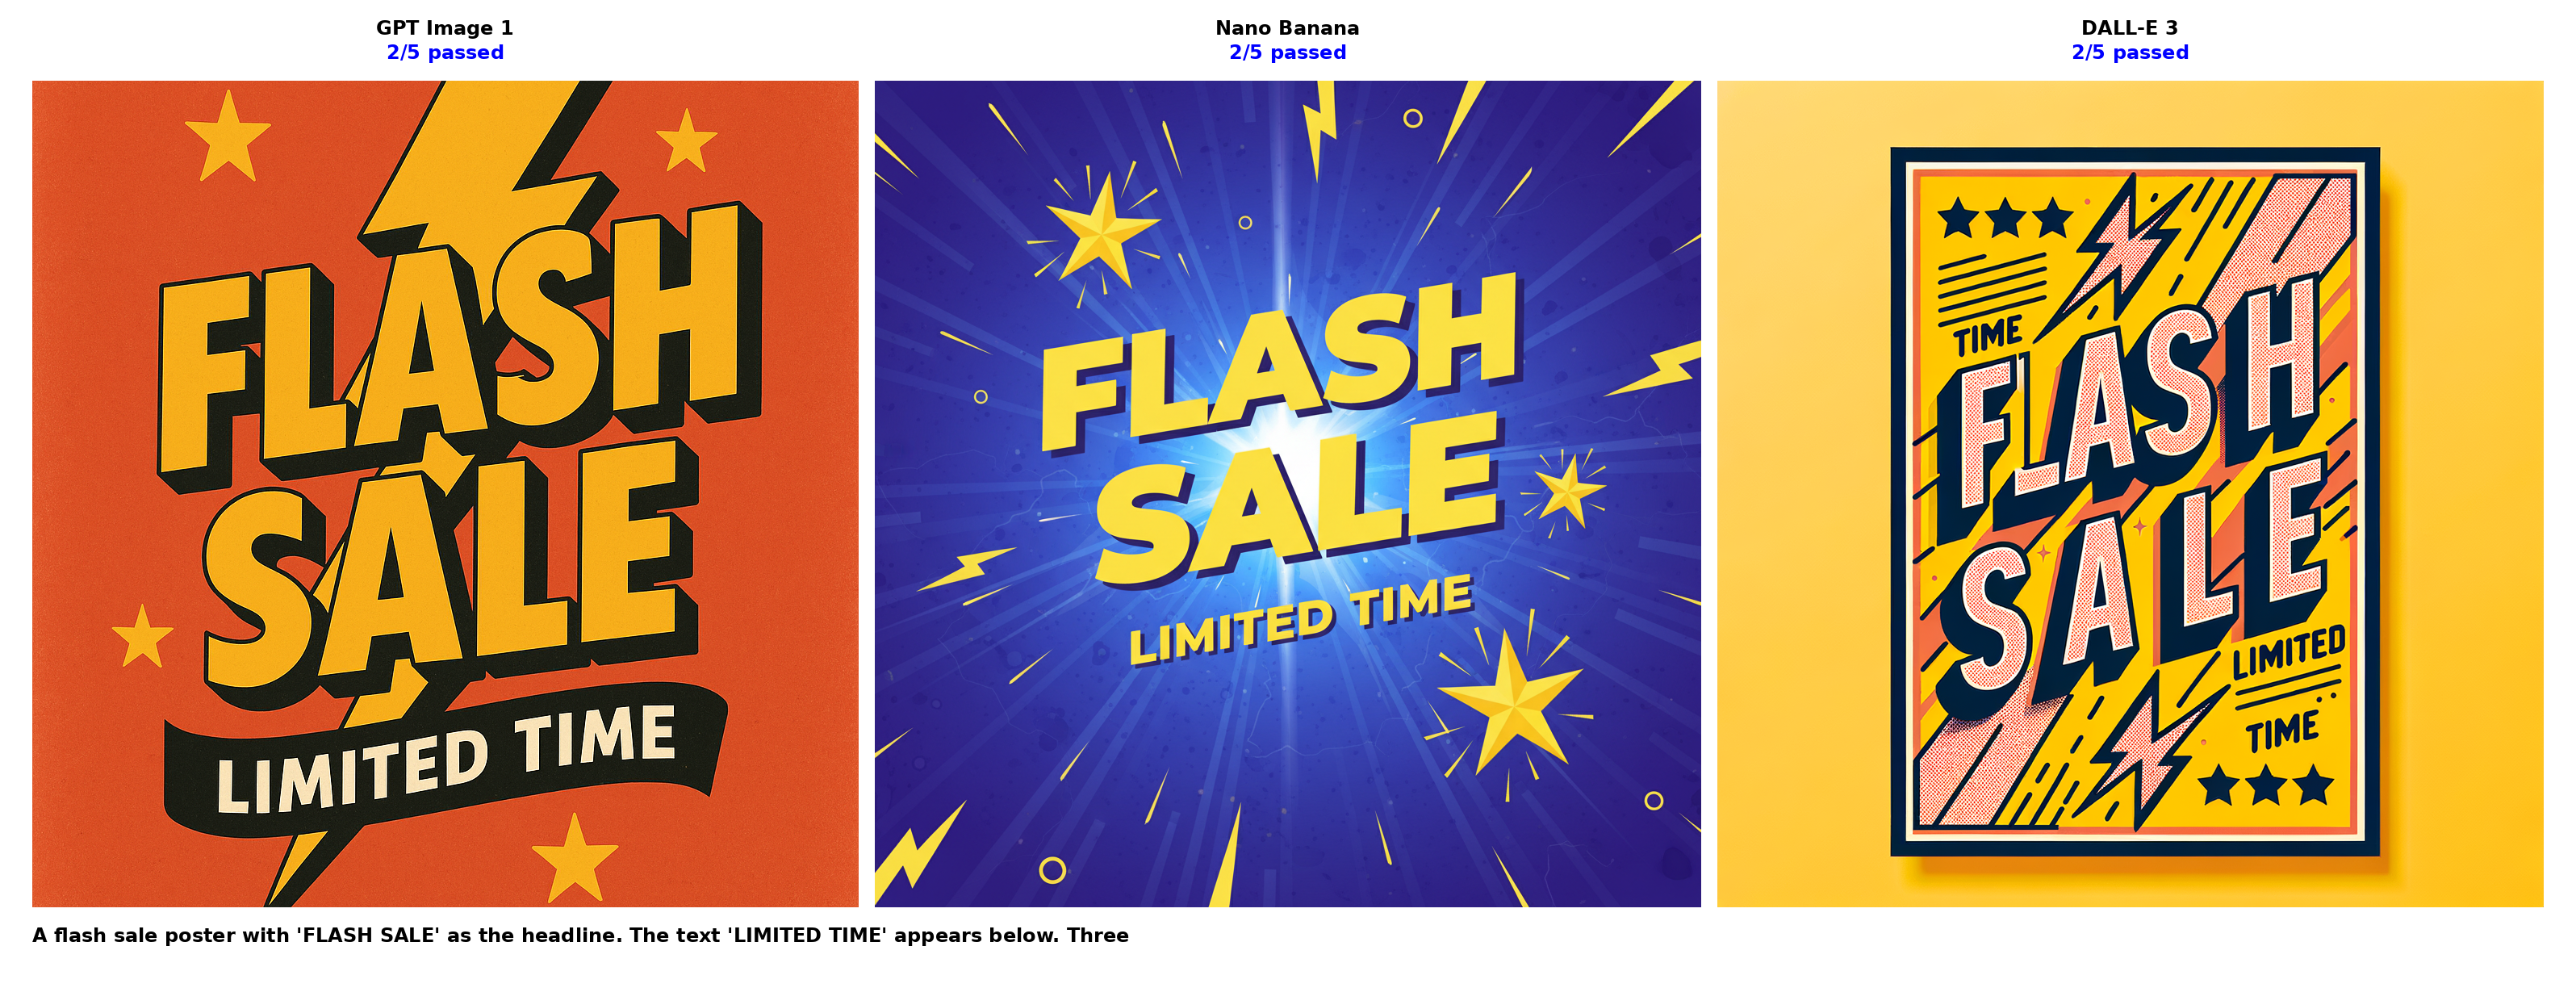
\includegraphics[width=0.95\textwidth]{paper_assets/case_studies/case_study_01_text_005.png}
\caption{Case Study 1: Text Rendering Comparison}
\label{fig:case1}
\end{figure}

\subsection{Case Study 2: Complex Composition}

\textbf{Prompt}: ``A photo of three blue mugs and two red plates on a wooden table. One of the blue mugs is tipped over. The largest blue mug is on the left side of the table, and the smallest red plate is on the right side.''

\textbf{Constraints}:
\begin{itemize}
    \item Count: 3 mugs, 2 plates
    \item Attribute: Blue mugs, red plates
    \item State: One mug tipped over
    \item Spatial: Largest mug left, smallest plate right
\end{itemize}

\textbf{Results}:
\begin{itemize}
    \item GPT Image 1: 2/6 constraints passed (spatial relationships correct)
    \item Nano Banana: 2/6 constraints passed
\end{itemize}

\textbf{Analysis}: Models successfully handle spatial relationships but struggle with precise counting and attribute verification.

\begin{figure}[H]
\centering
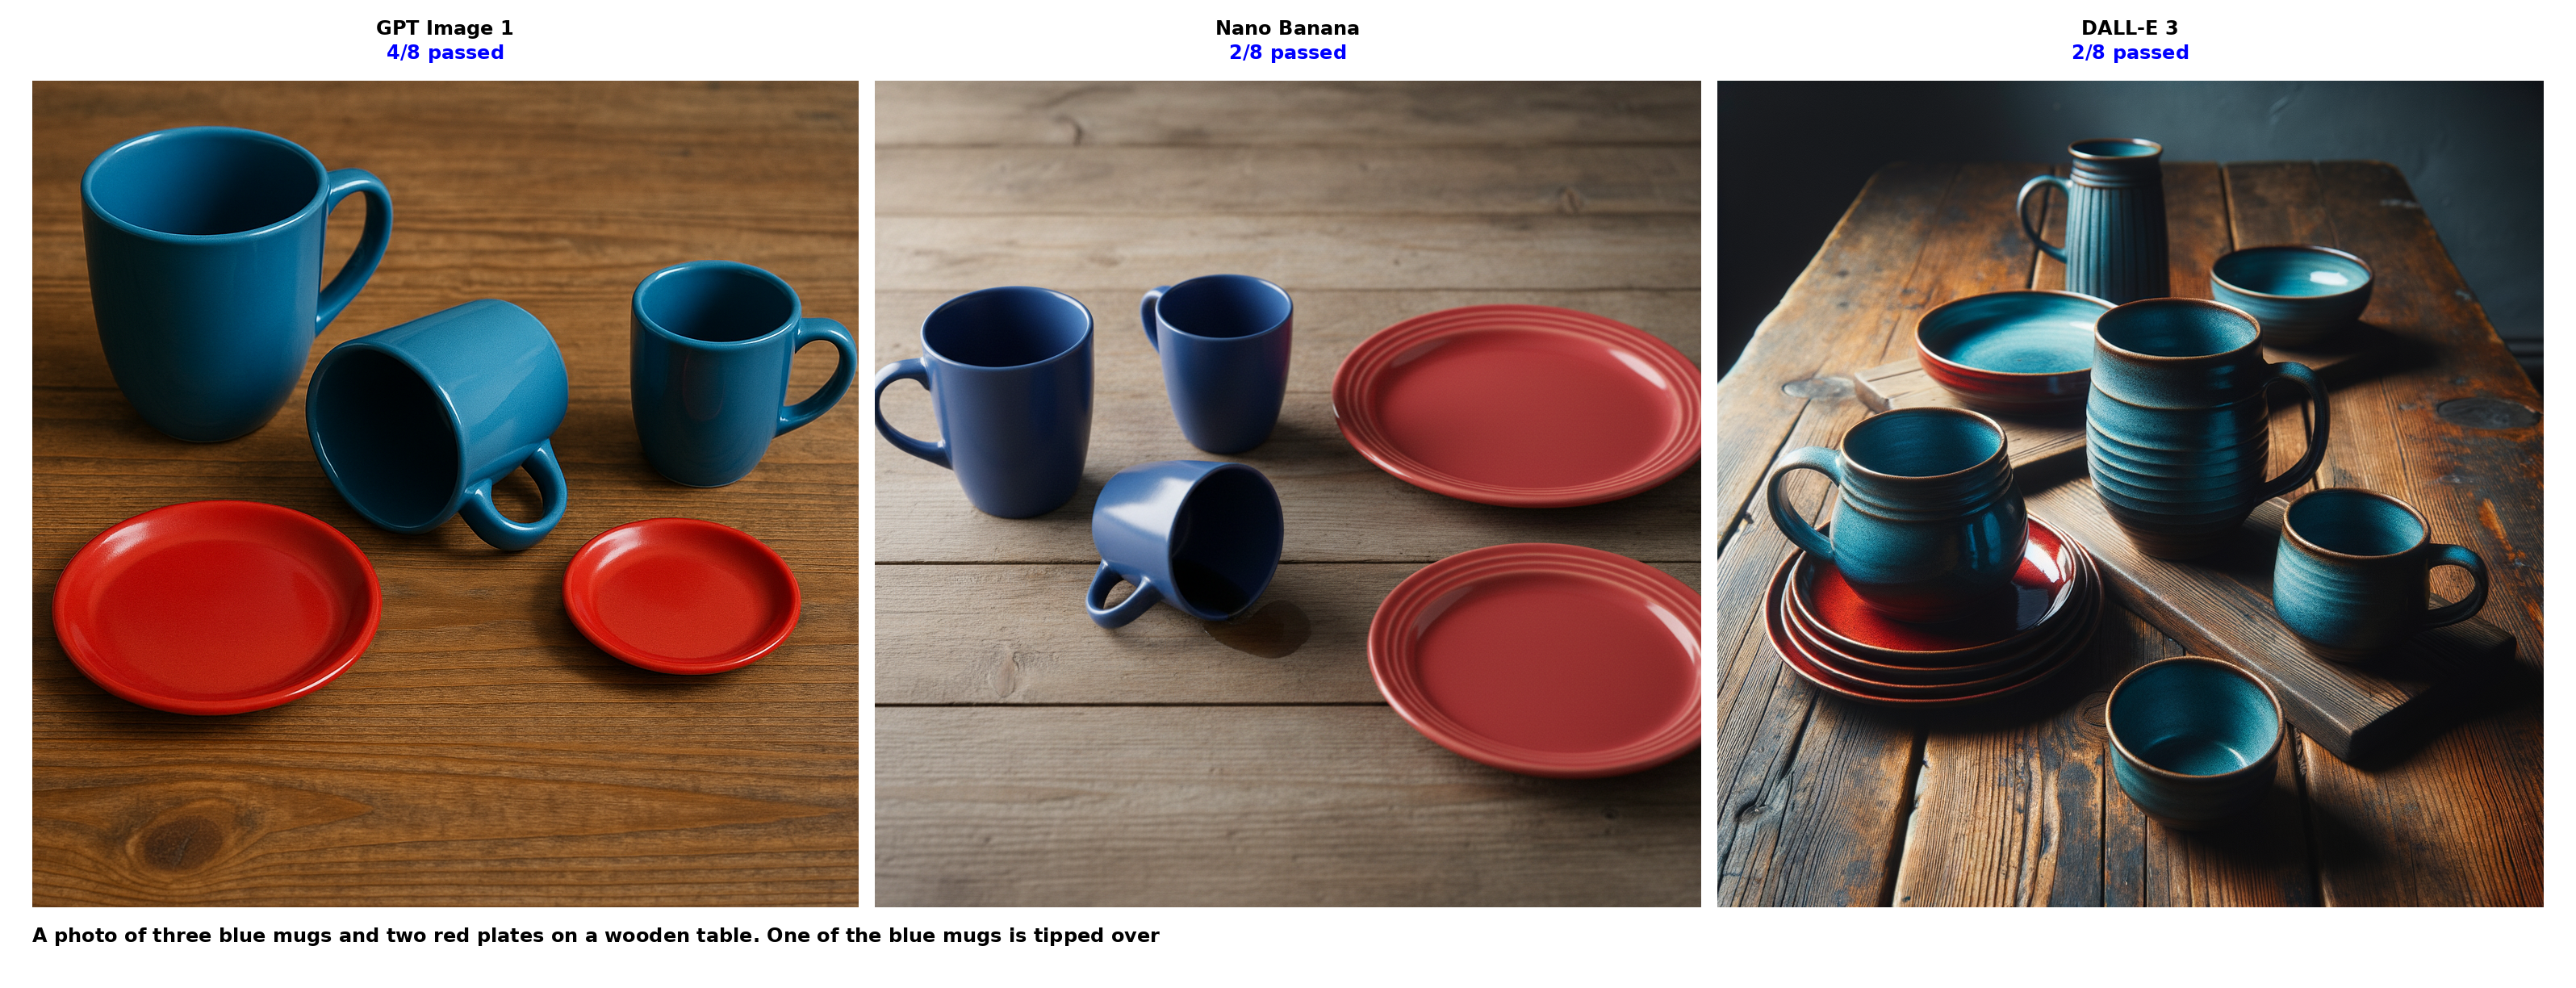
\includegraphics[width=0.95\textwidth]{paper_assets/case_studies/case_study_02_comp_001.png}
\caption{Case Study 2: Complex Composition Comparison}
\label{fig:case2}
\end{figure}

\subsection{Case Study 3: CSP Constraint}

\textbf{Prompt}: CSP task with numeric relationships

\textbf{Results}:
\begin{itemize}
    \item GPT Image 1: Passed (100\%)
    \item Nano Banana: Passed (95\%)
\end{itemize}

\textbf{Analysis}: Strong performance on mathematical constraints demonstrates effective OCR and numeric parsing capabilities.

\begin{figure}[H]
\centering
\includegraphics[width=0.95\textwidth]{paper_assets/case_studies/case_study_03_csp_01_numbers_row.png}
\caption{Case Study 3: CSP Constraint Comparison}
\label{fig:case3}
\end{figure}

\section{Cost and Latency Analysis}

\subsection{API Costs}

\begin{table}[H]
\centering
\caption{API Cost Analysis}
\label{tab:costs}
\begin{tabular}{lccc}
\toprule
\textbf{Model} & \textbf{Images} & \textbf{Cost/Image} & \textbf{Total Cost} \\
\midrule
GPT Image 1 & 47 & \$0.040 & \$1.88 \\
Nano Banana & 47 & \$0.005 & \$0.24 \\
DALL-E 3 & 11 & \$0.040 & \$0.44 \\
\bottomrule
\end{tabular}
\end{table}

\begin{figure}[H]
\centering
\includegraphics[width=0.9\textwidth]{paper_assets/figures/cost_performance_scatter.png}
\caption{Cost-Performance Trade-off Analysis}
\label{fig:cost_perf}
\end{figure}

\subsection{Cost-Performance Analysis}

Based on estimated costs and performance:
\begin{itemize}
    \item \textbf{Most Cost-Effective}: Nano Banana (\$0.24 for 47 images, 54.7\% pass rate)
    \item \textbf{Best Performance}: GPT Image 1 (\$1.88 for 47 images, 58.1\% pass rate)
    \item \textbf{Cost per Passed Constraint}: GPT Image 1: ~\$0.019; Nano Banana: ~\$0.003
\end{itemize}

\section{Limitations and Future Work}

\subsection{Current Limitations}

\begin{enumerate}
    \item \textbf{Incomplete DALL-E 3 Evaluation}: API billing limits prevented full evaluation
    \item \textbf{Limited Human Evaluation}: Primarily automated metrics; human preference scores not included
    \item \textbf{Cost/Latency Metrics}: Not systematically tracked in current evaluation
    \item \textbf{In-Painting Evaluation}: Not included in current benchmark (future addition)
\end{enumerate}

\subsection{Future Directions}

\begin{enumerate}
    \item Expand dataset: Add more prompts, especially for in-painting and out-painting tasks
    \item Human evaluation: Incorporate human preference scores and compositional accuracy ratings
    \item Cost analysis: Systematic tracking of API costs and generation latency
    \item Tool usage analysis: Evaluate model selection of generation vs. editing tools
    \item Trajectory visualization: Analyze multi-step generation processes
    \item Additional models: Evaluate Midjourney, Stable Diffusion 3, and other models
\end{enumerate}

\section{Conclusion}

The Visual Instruction Following Evaluation Benchmark (VIF-Eval) provides a comprehensive framework for assessing generative visual models beyond simple prompt adherence. Our evaluation of three state-of-the-art models reveals:

\begin{enumerate}
    \item \textbf{Strengths}: Models excel at spatial relationships, character consistency, and constraint satisfaction problems
    \item \textbf{Weaknesses}: Critical limitations in text rendering (12-13\% pass rate) and precise counting (17-31\% pass rate)
    \item \textbf{Comparability}: GPT Image 1 and Nano Banana show similar overall performance (54-58\% pass rates)
    \item \textbf{Cost-Efficiency}: Nano Banana provides significantly better cost-performance ratio
\end{enumerate}

The benchmark establishes a foundation for systematic evaluation of visual instruction following capabilities and provides actionable insights for model improvement. Future work should expand the dataset, incorporate human evaluation, and track cost/latency metrics to provide a complete assessment framework.

\newpage
\section*{Appendix A: Dataset Statistics}

\begin{itemize}
    \item Total Prompts: 47
    \item Total Constraints: 167-172 (varies by model)
    \item Constraint Types: 11 distinct types
    \item Categories: 7 categories
    \item Average Constraints per Prompt: 3.5
\end{itemize}

\section*{Appendix B: Evaluation Methodology Details}

Detailed evaluation logic for each constraint type is documented in \texttt{evaluation\_logic.txt}. Key evaluation methods include:

\begin{itemize}
    \item CLIP-based scoring for composition constraints
    \item OCR-based text extraction and validation
    \item Computer vision metrics (SSIM, edge detection, object detection)
    \item Face recognition for character consistency
    \item Mathematical constraint validation for CSP tasks
\end{itemize}

\end{document}
